\subsection{Il processo NLP}
Il processo di language processing deve, utilizzando una decomposizione analoga, generare una progressiva rimozione degli elementi di ambiguità partendo da un testo. Il suo obiettivo, pertanto, è quello di prendere un testo e attraverso una serie di trattamenti, in una cascata deterministica che decompone le fasi di analisi, produrre un’interpretazione del testo e rispondere al comando ricevuto con la pianificazione di un’azione da compiere.
La decomposizione si suddivide nelle fasi mostrate nella Figura \ref{fig:processo_nlp} a pagina \pageref{fig:processo_nlp}):
\begin{itemize}
    \item \textbf{Analisi lessicale}: Il testo viene sottoposto a una scansione per trovare le parole chiave o comunque i termini principali del discorso. Questa operazione avviene tramite un algoritmo detto \textbf{analizzatore lessicale}.
    Il testo viene suddiviso in frasi e parole prendendo come riferimento dei caratteri separatori, in genere lo spazio \textit{blank} e i segni di punteggiatura. 
    Una volta ottenuto l'insieme dei termini (\textit{token}) del testo, si analizzano per estrarre tutte le proprietà (\textit{feature}) che il linguaggio assegna a quella parola (la sua categoria grammaticale, se essa è nome, se è un numero, ecc.).
    
    Un testo senza \textit{stop-word} può essere ulteriormente normalizzato tramite un algoritmo di \textbf{stemming} che riduce le parole alla loro forma flessa (\textit{radice}). Si riduce così il numero delle varianti nel documento.
    
    \begin{figure}[hbt!]
        \centering
        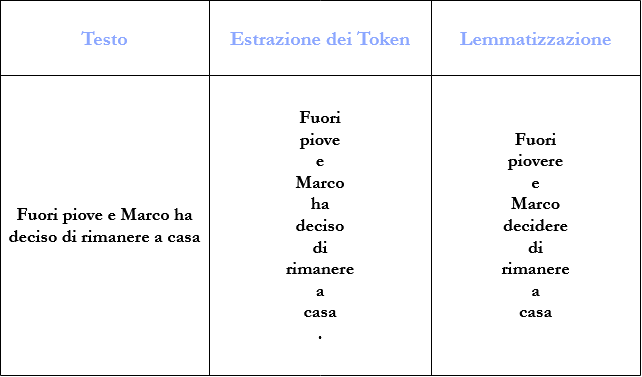
\includegraphics[width=0.8\textwidth]{img/analisi_lessicale.png}
        \caption{Analisi Lessicale}
        \label{fig:analisi_lessicale}
    \end{figure}
    
    \item \textbf{Analisi sintattica}: applica alle sequenze di token, ottenute tramite l’analisi lessicale, i principi della grammatica che genera il linguaggio nel quale è stato scritto il testo. Generalmente produce una struttura ad albero dove ad ogni nodo corrisponde o una parola o un costituente linguistico (frammento di frase), al quale corrisponderà una collocazione in una struttura gerarchica che nella sua radice copre l’intera frase. Si può dire che l’albero è la descrizione di tutte le relazioni grammaticali vigenti nella sequenza dei token in ingresso.
    L'insieme delle regole della sintassi prende nome di \textbf{regole di produzione} ed e strettamente collegato alla lingua.
    
    \begin{figure}[hbt!]
        \centering
        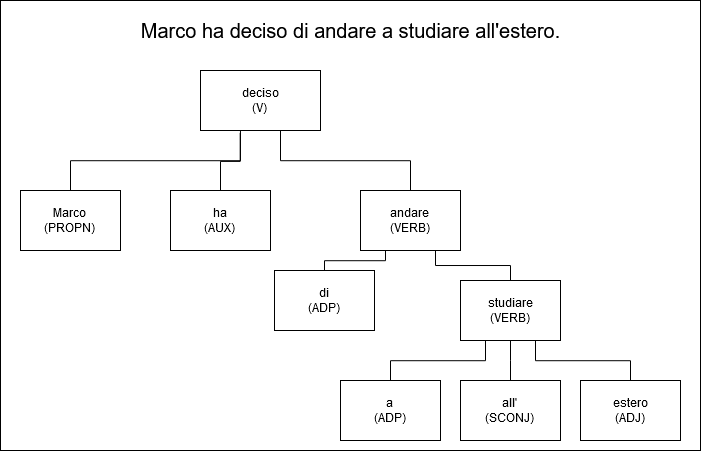
\includegraphics[width=0.8\textwidth]{img/analisi_sintattica.png}
        \caption{Analisi Sintattica}
        \label{fig:analisi_sintattica}
    \end{figure}
    
    \item \textbf{Analisi semantica}: si occupa di dare una spiegazione che descriva la relazione tra la frase e il mondo di riferimento (il "world model" nella figura \ref{fig:processo_nlp}).  L'analisi semantica è, pertanto, la ricerca del significato di un termine o di una frase. Non è sempre facile trovare il senso giusto delle parole. Spesso i termini hanno più significati (\textit{polisemici}) e occorre trovare quello giusto. Questo processo di selezione delle accezioni è detto \textbf{disambiguazione}. Le relazioni tra i concetti e i \textit{synset} consentono di costruire una struttura a rete detta \textbf{ontologia}. 
    In particolare si lavora su due livelli semantici differenti:
    
    \textbf{Semantica Lessicale}: studia il significato delle singole parole o di più termini, ovvero catene di parole il cui significato è diverso dalla somma dei significati delle singole parole (e.s. \textit{uscita d’emergenza}).
    
    \textbf{Semantica Frasale}: studia il significato di una frase, ponendo l’attenzione sulle interazioni tra i significati a livello delle parole. Prendiamo queste due frasi: \textit{Maria ha paura} vs. \textit{Maria sta giocando}. Maria ha lo stesso ruolo sintattico nei due casi (quello di soggetto) ma ha un diverso ‘ruolo semantico’: ha un ruolo attivo nell’attività di giocare, ma non nel caso di avere paura, che identifica uno stato emotivo che Maria vive involontariamente.
    
    A seconda del tipo di informazioni che si vogliono ottenere dai dati, è possibile usare una delle due tecniche di analisi semantica: \textit{text classification} o \textit{text extraction}. In particolare, in questa tesi sono stati trattati due task appartenenti alle queste due tecniche: \textbf{Topic Classification} per la Text Classification ed \textbf{Named Entity Recognition} per la Entity Extraction.
    
    \begin{figure}[hbt!]
        \centering
        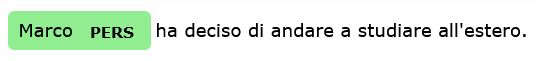
\includegraphics[width=0.8\textwidth]{img/analisi_semantica.png}
        \caption{Analisi Semantica: esempio di Named Entity Recognition}
        \label{fig:analisi_semantica}
    \end{figure}
    
    \item \textbf{Analisi pragmatica}: La dimensione pragmatica dell’analisi linguistica, secondo il filosofo americano Charles W. Morris, riguarda quegli aspetti che concernono l’azione indotta dall’uso del linguaggio. Studia il parlare in quanto forma di agire linguistico all’interno di una data situazione comunicativa. Molti enunciati, ad esempio, non veicolano informazioni, ma equivalgono ad azioni: “Scusami”, “Prometto”, “Si, lo voglio”, ecc.
    
    Nella forma logica, il significato delle parole viene messo in corrispondenza con il livello pragmatico (ovvero “cosa si aspetta da me la persona?”, “qual è  il suo scopo?”) e quindi, da un punto di vista applicativo, il sistema reagisce.  Le parole della forma logica rappresentano degli scopi e, dal punto di vista del modello, interpretare la forma logica e trasformarla in un’azione significa interpretare l’ultimo livello dell’analisi che è quello degli scopi che per l’utente ha quel testo.
\end{itemize}

\begin{figure}[hbt!]
    \centering
    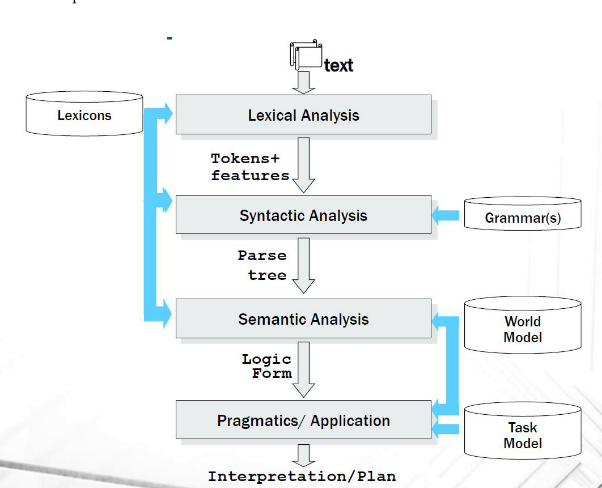
\includegraphics[width=1\textwidth]{img/processo_nlp.png}
    \caption{Il processo NLP}
    \label{fig:processo_nlp}
\end{figure}